\documentclass{article}
\usepackage[ruled, linesnumbered]{algorithm2e}
\def\showtopic{Numerical Analysis}
\def\showtitle{Lab 3:Nonlinear Solver}
\def\showabs{Lab 3}
\def\showauthor{Ting Lin, 1700010644}
\def\showchead{LIN}
\usepackage{amsmath, amsfonts, amsthm}

\usepackage{graphicx, epstopdf}
\usepackage{color}
\usepackage{geometry, graphicx}
\usepackage{algorithm, algorithmic}
\usepackage{bm}
\usepackage{multirow}
\usepackage{ulem}
\geometry{left = 5em, right = 5em}
\usepackage{listings}
\usepackage{xcolor}
%% notation macro
\newcommand{\F}{\mathcal F}
\newcommand{\T}{\mathcal T}
\newcommand{\I}{\mathcal I}
\newcommand{\U}{\mathcal U}
\newcommand{\R}{\mathbb R}
\renewcommand{\P}{\mathcal P}
\newcommand{\uP}{ \mathcal \uline P}
\newcommand{\B}{\mathcal B}
%\newcommand{\R}{\mathbb R^2}
\newcommand{\Z}{\mathbb Z}
\newcommand{\C}{\mathbb C}
\newcommand{\laplacian}{\triangle}
\newcommand{\grad}{\nabla}
\renewcommand{\div}{\textrm{div~}}

\newcommand{\diff}[2]{\frac{\partial #1}{\partial #2}}
\newcommand{\difff}[3]{\frac{\parial #1^2}{\partial #2 \partial #3}}
\newcommand{\diFF}[2]{\frac{\partial #1^2}{\partial^2 #2}}
\newcommand{\diam}{\text{ diam }}
%% non-noation macro
\newcommand{\IN}{\text{  in  }}
\newcommand{\ON}{\text{  on  }}
\newcommand{\st}{\text{s.t.  }}
\newcommand{\tbc}{{\color{red}[TBC]}}

%% enviorment
\newtheorem{proposition}{Proposition}
\newtheorem{definition}{Definition}
\newtheorem{corollary}{Corollary}
\newtheorem{remark}{Remark}



\title{\textbf{\showtitle}}
\author{\showauthor}
\usepackage{indentfirst}
\usepackage{fancyhdr}  
\pagestyle{fancy}
\lhead{\textbf {\showtopic} }
\chead{} 
\rhead{\textbf {\showabs} }
\lfoot{} 
\cfoot{\thepage}
\rfoot{} 
\renewcommand{\headrulewidth}{0.4pt} 
\DeclareMathOperator{\size}{size}
\begin{document}
	\maketitle
	\thispagestyle{fancy}
	\tableofcontents
	
	\section*{}

In this report we introduce the FFT algorithm, and implements a filter based on FFT by C++. 

\section{FFT Algorithm}
The FFT algorithm is developed as a fast solver of discrete fourier transform:
We set $c = \hat a$ if 
$$c_k = \sum_{j=0}^{N-1} a_j e^{-2\pi ijk/N}.$$
By inverse formula or direct calculation we can obtain the inverse DFT
$$a_k = \sum_{j=0}^{N-1} c_j e^{-2\pi ijk/N}.$$
For simplicity we only consider the case of $N = 2^m$. 

The basic idea is from Danielson--Lanczos algorithm. 
Set 
\begin{equation}
\begin{split}
P(x) =& a_0 + a_1x + \cdots a_Nx^{N-1} \\ 
 =& P_e(x^2) + xP_o(x^2)
\end{split}
\end{equation}
Define $\omega_k = \exp(-2\pi i/k)$, when $j=0,\cdots, \frac N2-1$, we have 
$$c_j = P_(\omega_N^{2j}) + \omega_N^jP_o(\omega_N^{2j})$$
$$c_{N/2+j} = P_(\omega_N^{2j+N}) + \omega_N^{j+N/2}P_o(\omega_N^{2j+N})$$
Notice that 
$$\omega_N^{2j} =\omega_N^{2j+N} =  \omega_{N/2}^j, \omega_N^{N/2 + j} = -\omega_{N}^j, $$
we have 
$$c_j = v_j + \omega_N^ju_j, c_{j+N/2} = v_j - \omega_N^j u_j$$
where $v_j = P_e(\omega_{N/2}^j), u_j = P_o(\omega_{N/2}^j)$

From this we define the D-L algorithm recursively
\begin{algorithm}[H]
	\caption{$c = \textbf{FFT}(a)$)}
	\begin{algorithmic}[1]
		\IF{$N:=\size(a)==1$}
		\STATE \Return $a$
		\ENDIF
		\STATE Compute $v_j = \textbf{FFT}(a(0:2:N-1)), u_j = \textbf{FFT}(a(1:2:N))$
		\STATE $e = \exp(-2\pi i/N), w = 1$
		\FOR{$j=0:N/2-1$}
		\STATE $c_j = v_j + wu_j$
		\STATE $c_{j+N/2} = v_j - wu_j$
		\STATE $w = w\cdot e$
		\ENDFOR
	\end{algorithmic}
\end{algorithm}

We only need replace $w = e = \exp(-2\pi i/N)$ by $w = e = \exp(2\pi i/N)$ to obtain the IFFT algorithm.

For practical concerning, we adopt a 2-stage FFT: re-ordering and assembling.

The main trick of re-ordering is computing the bit-reverse of an index.
\begin{algorithm}[H]
	\caption{$\textbf{REORDER}(a)$}
	\begin{algorithmic}[1]
		\STATE $j=0$ (denote the bit-reverse result), $N = \size(a)$
		\FOR{$i=0:N$}
		\IF{$i<j$}
		\STATE swap($a_i, a_j$)
		\ENDIF
		\STATE $l = k>>1, j = j\wedge l$
		\WHILE{$j<l$}
		\STATE $l=l>>1$
		\STATE $j=j\wedge l$
		\ENDWHILE
		\ENDFOR
		\end{algorithmic}
\end{algorithm}
Here $\wedge, >>$ is bit operation from C.
After re-ordering, assembling step is quite easy.
\begin{algorithm}[H]
	\caption{$\textbf{ASSEMBING}(a)$}
	\begin{algorithmic}[1]
		\STATE Copy $a$ to $c$.
		\STATE $m=2, n = \size(a)$
		\WHILE{$m\le n$}
		\STATE{$e = \exp(-2\pi i/N)$} \COMMENT{//$e = \exp(2\pi i/N)$ for ifft case}
		\FOR{$k=0:m:n-m$}
		\STATE $w=1$
		\FOR{$j=0:m/2-1$}
		\STATE $t = w*a_{k+j+m/2}, u = a_{k+j}$
		\STATE $a_{k+j} = u + t, a_{k+j+m/2} = u-t$
		\ENDFOR
		\ENDFOR
		\STATE $m = 2m$
		\ENDWHILE
		\STATE \COMMENT{//$a_i = a_i/n$ for ifft case}
		\end{algorithmic}
	\end{algorithm}

After this, we obtain the whole (inplace) FFT.
\begin{algorithm}[H]
	\caption{$\textbf{FFT}^*(a)$}
	\begin{algorithmic}[1]
		\STATE \textbf{RE-ORDERING}$(a)$
		\STATE \textbf{ASSEMBLING}$(a)$
		\end{algorithmic}
\end{algorithm}
By considering comments in assembling, we obtain the IFFT* algorithm.




\section{Numerical Result and Discussions}
\subsection{Filtering}
We use FFT to implement the filtering algorithm. Suppose $a$ is a N-array. For given threshold $m$, we set $c_i = (\hat a)_i$ if $|i|\ge M$ otherwise $c_i = 0$. Then we denote $\mathcal F_m a = \breve{c}$.

Mathematically, the filtering operator preserves all the low-frequency information and exclude the high-frequency one, this makes the function less oscillatory when function is smooth enough. 
\subsection{Numerical Result}
We show an non-trivial example when the function is not continuous. Set $f(t)= \exp(-t^2/10)(sin(2t)+2cos(4t)+0.4sin(t)sin(50t))$, and we choose $f(2\pi k/256) (k = 0,1,\cdots, 255)$ to discretize it .
We plot for $m = 2,3,4,5,6,10,20,30,40,50$.
\begin{figure}
	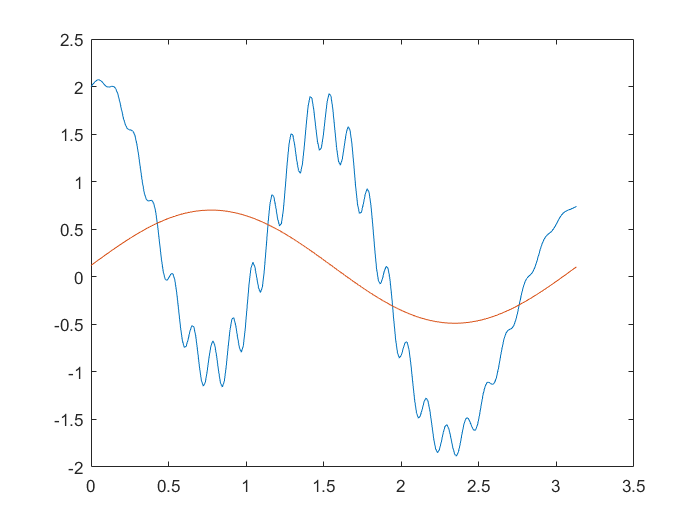
\includegraphics[scale=.5]{../res1.png}
	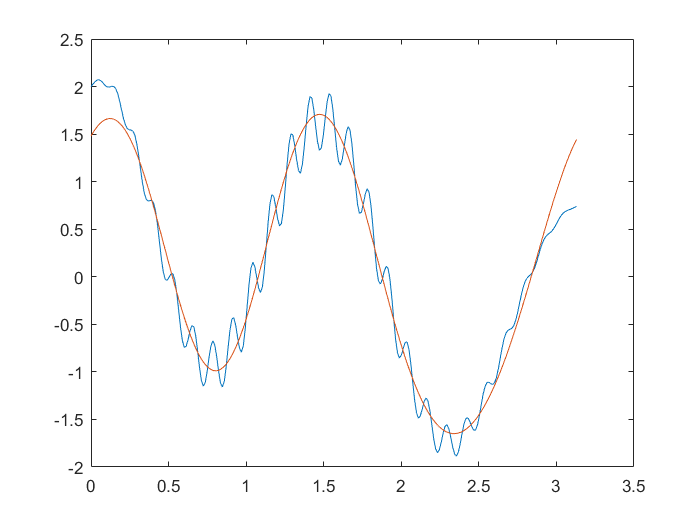
\includegraphics[scale=.5]{../res3.png}
	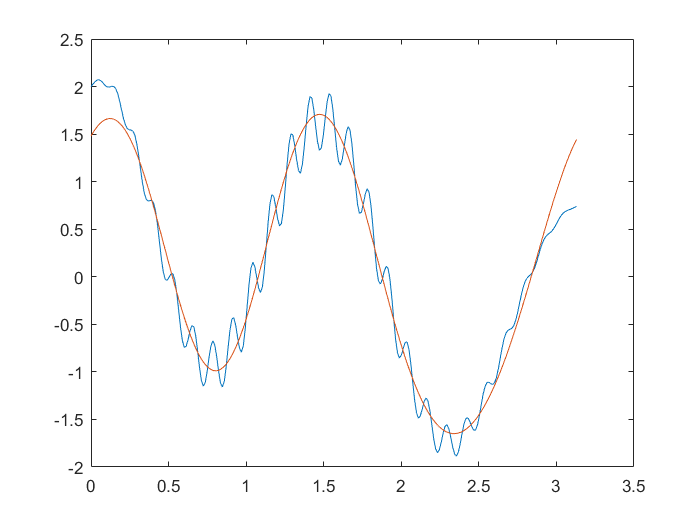
\includegraphics[scale=.5]{../res4.png}
	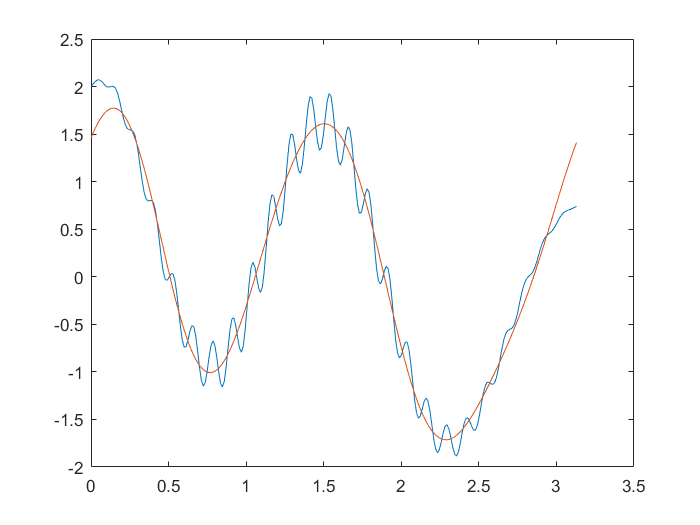
\includegraphics[scale=.5]{../res5.png}
	\caption{m = 2,3,4,5}
\end{figure}
\begin{figure}
	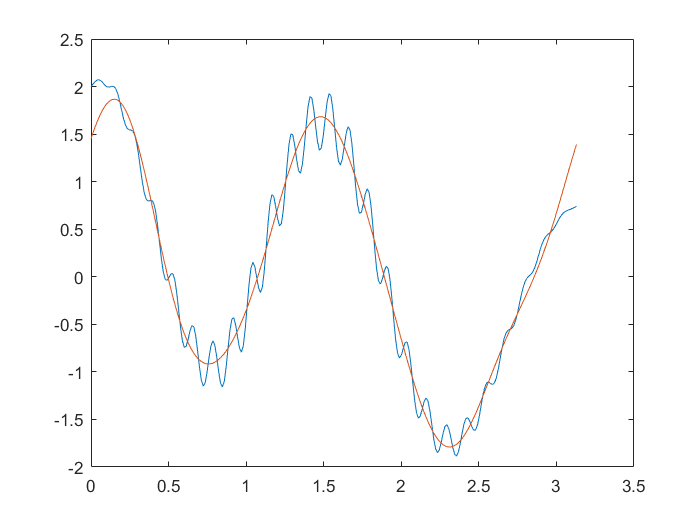
\includegraphics[scale=.5]{../res6.png}
	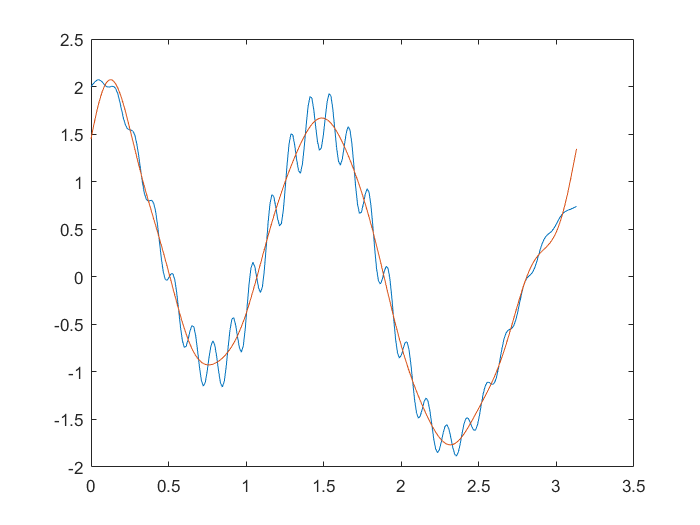
\includegraphics[scale=.5]{../res10.png}
	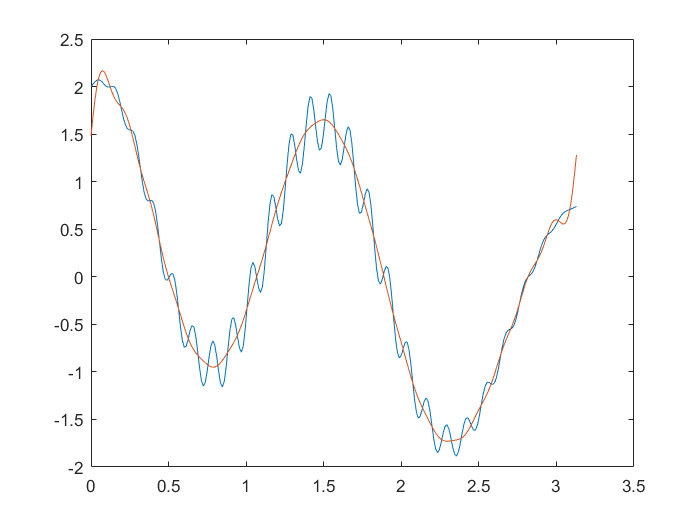
\includegraphics[scale=.5]{../res20.png}
	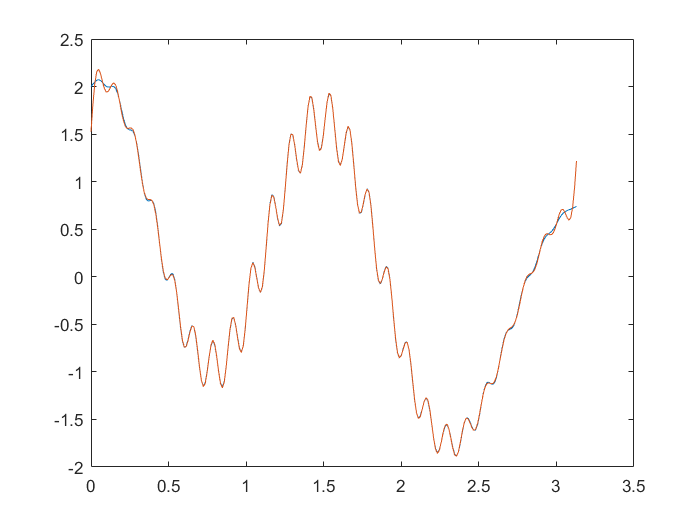
\includegraphics[scale=.5]{../res30.png}
	\caption{m = 6,10,20,30}
\end{figure}
\begin{figure}
	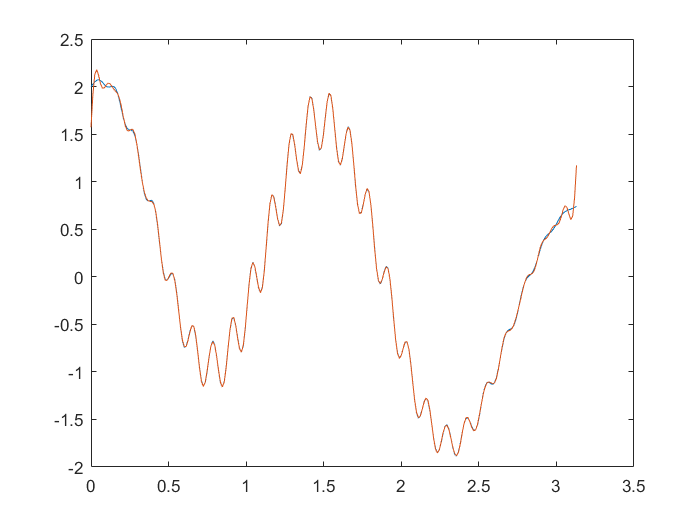
\includegraphics[scale=.5]{../res40.png}
	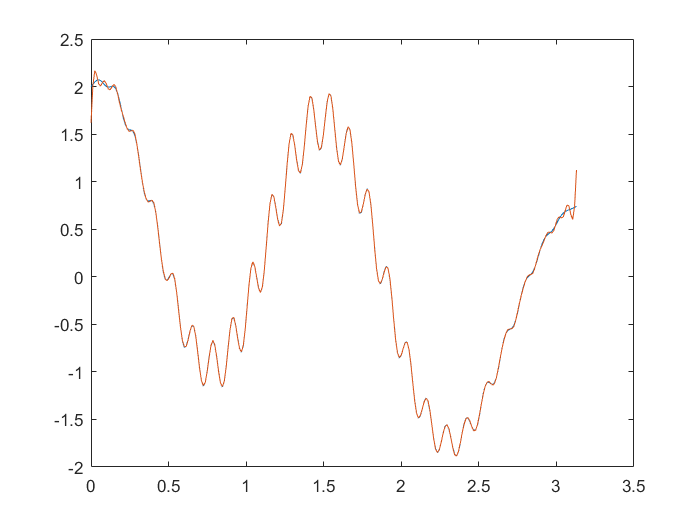
\includegraphics[scale=.5]{../res50.png}
	\caption{m = 40,50}
\end{figure}
Notice that the gibbs phenomenon is easy to see. The gibbs phenomenon is caused by the jump in point $0$.
Furthermore, the approximation result has significant improvement when $m$ increases from 20 to 30. Hence it will be better to a sparse frequency approximation then just filtering, and the behavior will be better.

\end{document}
















Escape special TeX symbols (%, &, _, #, $)